\documentclass[tikz,border=10pt]{standalone}
\usepackage{amsmath}
\usepackage{amssymb}
\usepackage{xcolor}
\usetikzlibrary{arrows.meta,decorations.pathreplacing}

\definecolor{predictoraccent}{HTML}{1F77B4}
\definecolor{responseaccent}{HTML}{FF7F0E}
\definecolor{pairedaccent}{HTML}{2CA02C}
\definecolor{couplingaccent}{HTML}{F2B01E}
\definecolor{textgray}{HTML}{30343B}

\tikzset{
  observed/.style={
    rectangle,
    minimum width=0.62cm,
    minimum height=0.54cm,
    inner sep=0pt,
    line width=0.7pt,
    draw=textgray!85,
  },
  predictor observed/.style={
    observed,
    fill=predictoraccent!42,
  },
  response observed/.style={
    observed,
    fill=responseaccent!48,
  },
  predictor mode/.style={
    rectangle,
    rounded corners=1.5pt,
    minimum width=1.15cm,
    minimum height=0.66cm,
    line width=0.8pt,
    draw=pairedaccent!90!black,
    fill=pairedaccent!22,
    text=textgray,
  },
  response mode/.style={
    rectangle,
    rounded corners=1.5pt,
    minimum width=1.15cm,
    minimum height=0.66cm,
    line width=0.8pt,
    draw=couplingaccent!85!black,
    fill=couplingaccent!32,
    text=textgray,
  },
  fan/.style={
    draw=textgray!48,
    line width=0.55pt,
  },
  coupling/.style={
    -{Latex[length=2.0mm,width=1.35mm]},
    draw=textgray!82,
    line width=0.9pt,
  },
  heading/.style={
    align=center,
    text=textgray,
    font=\bfseries\large,
  },
  annotation/.style={
    align=center,
    text=textgray!82,
    font=\small,
  },
}

\begin{document}
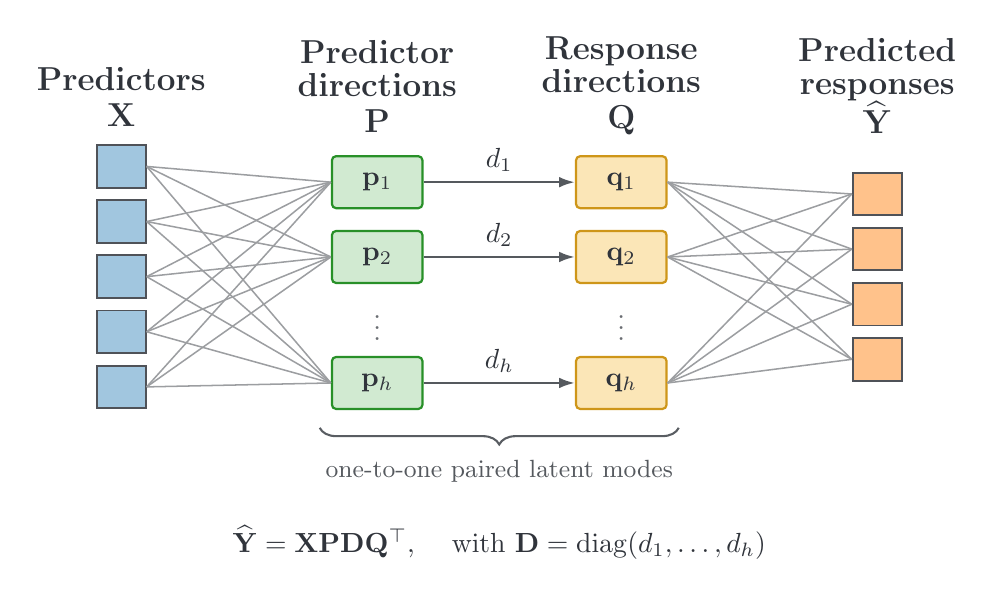
\begin{tikzpicture}[x=1cm,y=1cm]
  % Observed predictor variables.
  \node[predictor observed] (x1) at (0, 1.60) {};
  \node[predictor observed] (x2) at (0, 0.90) {};
  \node[predictor observed] (x3) at (0, 0.20) {};
  \node[predictor observed] (x4) at (0,-0.50) {};
  \node[predictor observed] (x5) at (0,-1.20) {};

  % Paired predictor and response directions.
  \node[predictor mode] (p1) at (3.25, 1.40) {$\mathbf{p}_1$};
  \node[predictor mode] (p2) at (3.25, 0.45) {$\mathbf{p}_2$};
  \node[text=textgray!72] (pdots) at (3.25,-0.35) {$\vdots$};
  \node[predictor mode] (ph) at (3.25,-1.15) {$\mathbf{p}_h$};

  \node[response mode] (q1) at (6.35, 1.40) {$\mathbf{q}_1$};
  \node[response mode] (q2) at (6.35, 0.45) {$\mathbf{q}_2$};
  \node[text=textgray!72] (qdots) at (6.35,-0.35) {$\vdots$};
  \node[response mode] (qh) at (6.35,-1.15) {$\mathbf{q}_h$};

  % Predicted response variables.
  \node[response observed] (y1) at (9.60, 1.25) {};
  \node[response observed] (y2) at (9.60, 0.55) {};
  \node[response observed] (y3) at (9.60,-0.15) {};
  \node[response observed] (y4) at (9.60,-0.85) {};

  % Predictor variables contribute to each predictor direction.
  \foreach \xnode in {x1,x2,x3,x4,x5}{
    \foreach \pnode in {p1,p2,ph}{
      \draw[fan] (\xnode.east) -- (\pnode.west);
    }
  }

  % Each response direction contributes to the predicted responses.
  \foreach \qnode in {q1,q2,qh}{
    \foreach \ynode in {y1,y2,y3,y4}{
      \draw[fan] (\qnode.east) -- (\ynode.west);
    }
  }

  % The diagonal map creates one-to-one paired latent modes.
  \draw[coupling] (p1.east) -- node[above, text=textgray] {$d_1$} (q1.west);
  \draw[coupling] (p2.east) -- node[above, text=textgray] {$d_2$} (q2.west);
  \draw[coupling] (ph.east) -- node[above, text=textgray] {$d_h$} (qh.west);

  % Layer labels and concise interpretation cues.
  \node[heading] at (0,2.48) {Predictors\\[-1pt]$\mathbf{X}$};
  \node[heading] at (3.25,2.62) {Predictor\\[-2pt]directions\\[-1pt]$\mathbf{P}$};
  %\node[annotation] at (3.25,1.44) {retained panorama\\[-2pt] rank $r_\pi$};
  \node[heading] at (6.35,2.62) {Response\\[-2pt]directions\\[-1pt]$\mathbf{Q}$};
  \node[heading] at (9.60,2.62) {Predicted\\[-2pt]responses\\[-1pt]$\widehat{\mathbf{Y}}$};

  \draw[decorate,decoration={brace,mirror,amplitude=6pt},line width=0.75pt,draw=textgray!80]
    (2.52,-1.72) -- (7.08,-1.72)
    node[midway,below=8pt,annotation] {one-to-one paired latent modes};

  \node[text=textgray, font=\normalsize] at (4.80,-3.17)
    {$\widehat{\mathbf{Y}}=\mathbf{X}\mathbf{P}\mathbf{D}\mathbf{Q}^{\top}$,
     \quad with $\mathbf{D}=\operatorname{diag}(d_1,\ldots,d_h)$};
\end{tikzpicture}
\end{document}
